% Ni-YSZ voxel damage operators -- manuscript
% Target: Journal of Power Sources (Elsevier, elsarticle, 5p two-column layout)
% Build: pdflatex manuscript && pdflatex manuscript
\documentclass[5p,times,twocolumn]{elsarticle}

\usepackage{lmodern}
\usepackage[T1]{fontenc}
\usepackage[utf8]{inputenc}
\usepackage{amsmath,amssymb}
\usepackage{graphicx}
\usepackage{booktabs}
\usepackage{siunitx}
\usepackage{microtype}
\usepackage[hidelinks]{hyperref}
\usepackage{xcolor}

\sisetup{detect-all, group-digits=none}
\graphicspath{{figs/}}

% A period after a lowercase letter makes LaTeX assume a sentence has ended and
% widen the following space, so "Fig.~\ref{}" and "et al." were setting too
% loose. frenchspacing makes inter-word and inter-sentence spacing uniform.
\frenchspacing

% Captions were sitting hard against their tables and figures.
\setlength{\abovecaptionskip}{9pt}
\setlength{\belowcaptionskip}{7pt}
\journal{Journal of Power Sources}

\newcommand{\Rni}{R_{\mathrm{Ni}}}
\newcommand{\Pspan}{P_{\mathrm{span}}}
\newcommand{\Preach}{P_{\mathrm{reach}}}
\newcommand{\Sspec}{S_{\mathrm{spec}}}
\newcommand{\nb}{\mathrm{nb}}

\begin{document}

\begin{frontmatter}

\title{Validation criteria that exclude their own mechanism: six failure
modes of voxel damage operators applied to Ni--YSZ tomograms}


\author[a]{Arnav Mehta}
\ead{amehta33@wisc.edu}
\address[a]{Department of Mechanical Engineering, University of Wisconsin--Madison, Madison, WI, USA}



\begin{abstract}
A simulation can satisfy every validity check its authors impose and still move
the microstructure away from the physics it represents. We show this for
voxel-scale damage operators on segmented tomograms, a standard way to simulate
degradation in solid oxide cell electrodes.

A coarsening rule invites one obvious criterion, that it should reduce
specific surface area monotonically. We pre-registered exactly that. On a 6-connected
lattice a single-voxel swap changes exposed area by exactly $2[\nb(a)-\nb(b)]$,
so the criterion is a comparison of neighbour counts, and it leaves a large
null space in which four in five accepted moves change the area by exactly
zero. On three FIB-SEM reconstructed Ni--YSZ anodes the operator satisfies
the criterion in full, area falling monotonically at exact volume conservation,
while triple-phase-boundary density rises three- to fivefold. The inflation is
localised rather than diffuse. Re-applying only the moves that touch the
nickel--zirconia contact reproduces all of it, while every other move together
gives $\times1.04$. Strict inequality
reduces the artifact without removing it. Surface area is the wrong invariant
to validate a coarsening rule against.

The same criterion excludes Rayleigh-type neck break-up, which needs a
transient area increase. No operator respecting it thinned a neck.

Four further modes are measured, each invisible on synthetic structures:
largest-component pruning makes the spanning fraction identically unity, so the
operator rewrites the denominator of the metric judging it; gates requiring
perfect pristine connectivity misrepresent electrodes carrying
\SIrange{1.2}{11.2}{\percent} disconnected nickel; a jittered lattice cuts at
one cross-section with zero variance where real networks fail at
\SIrange{0.5}{3}{\percent} of throats. One check costs a line of code, since an operator whose TPB retention exceeds
unity is roughening rather than coarsening.
\end{abstract}

\begin{keyword}
solid oxide cell \sep Ni--YSZ anode \sep FIB-SEM tomography \sep
percolation \sep triple-phase boundary \sep microstructural degradation
\end{keyword}

\end{frontmatter}

%======================================================================
\section*{Nomenclature}
%======================================================================

\begingroup\small
\begin{tabular}{@{}l@{\hspace{0.9em}}p{0.60\columnwidth}@{}}
$\nb(x)$ & nickel 6-neighbours of voxel $x$, centre excluded \\
$\Delta A$ & change in exposed nickel area per swap, in faces \\
$\Sspec$ & specific surface area, faces per nickel voxel \\
$\Pspan$ & nickel fraction in a face-to-face spanning cluster \\
$\Preach$ & nickel fraction reachable from one face \\
$\Rni$ & spanning-cluster voxels over \emph{pristine} nickel voxels \\
TPB & triple-phase boundary length per volume \\
$\Phi_{\mathrm{Ni}}$ & nickel volume fraction \\
$n$ & damage intensity, in rounds \\
$\rho$ & Spearman rank correlation coefficient \\
\end{tabular}
\endgroup



%======================================================================
\section{Introduction}
%======================================================================

Nickel--yttria-stabilised-zirconia cermet anodes lose performance in service
through microstructural change. Nickel coarsens and can lose the percolating
network that carries electronic current \cite{simwonis2000}; the ceramic
scaffold fractures under redox cycling \cite{sarantaridis2007}; and the
triple-phase boundary (TPB), the one-dimensional locus where nickel, zirconia
and pore meet and where the electrochemical reaction proceeds, is lost as the
nickel agglomerates \cite{monaco2019}. All three are geometric
processes acting on a
microstructure that FIB-SEM and X-ray nano-tomography now resolve routinely,
which makes a particular computational strategy very attractive. One takes a
segmented tomogram, applies a damage operator to the label field, and tracks
how connectivity and TPB evolve.

The strategy is attractive because it is cheap and because it acts on the same
data structure the experimentalist already has. It is also, as far as we can
tell, less examined than the continuum alternative. Phase-field treatments of
Ni coarsening in this system have been developed and progressively validated
over more than a decade, from the early three-phase simulations on
experimentally acquired anode functional layers \cite{chen2011}, through
validation against time-dependent ex-situ tomography of one specimen imaged
pristine and after annealing \cite{trini2021}, to
quantitative simulations initialised on ptychographic
nano-tomograms with measured thermophysical parameters \cite{yang2023} and
multiphase-field models coupled to transmission-line performance estimates on
FIB-SEM reconstructions \cite{hoffrogge2023}. Discrete methods have been
applied on the fabrication side, where a Potts kinetic Monte Carlo model of
NiO--YSZ sintering was calibrated against FIB-SEM microstructure and validated
on volume fraction, specific surface area and triple-phase boundary density
\cite{zhou2023}. Carrying that machinery over to degradation is less an open
gap than an obvious next step, since it is the same free-energy formulation
run under different driving conditions.

What is less examined is what happens when a discrete operator is instead
assembled for the degradation problem directly, and how the conventions that
surround such an operator interact with each other. Three matter here, the
connectivity metric, the qualification gate on the test structure, and the
validity criterion on the operator itself. We did not adopt the established formulation, and this
paper is in part an account of what that cost.

This paper is that account, and it is negative in its first-order result. We
set out to identify which damage mechanism reproduces a measured degradation
signature in three Ni--YSZ anodes, and we did not find one. One operator
reached a mechanism verdict on real tomograms, and reversed the measured
ordering rather than reproducing it. Three more were run to a conclusion on a
synthetic platform that we then had to disqualify. Four further routes closed
before any mechanism test was reached, two because the operator failed its own
validity gate and two because the data cannot pose the question. Along the way
six specific ways in which this class of simulation
silently misleads were identified and measured. We think the second finding is
the more useful one, and the paper is organised around it, but the two are not
separable, since the failure modes were found by running the programme that
failed, and they are reported in the order in which the work forced us to
confront them.

The experimental target is unusually sharp and runs against intuition. Across
the anode series of Pecho and co-workers \cite{pecho2015transport,pecho2015tpb}
the finest microstructure retains nickel percolation worst while
retaining TPB best (Fig.~\ref{fig:signature}, Table~\ref{tab:target}).
A coarsening argument predicts the first half, because by Herring's scaling
laws the
time to produce a geometrically similar change scales as a power of the
particle size \cite{herring1950}, so the finest structure should coarsen
fastest and lose its network first. It does not obviously predict the second
half, in which the same anode preserves four fifths of its reaction sites.

Two cautions travel with that target throughout this paper, and both follow
from how the data were acquired rather than from how they were analysed.
Medium versus coarse is not resolved on the nickel side, since the ordering
flips
depending on whether percolation is defined by two-face spanning or by
reachability from one face. And the published TPB series is not monotone,
since coarse (0.608) exceeds medium (0.586). Only the two-level statements,
\textbf{fine retains nickel percolation worst} and \emph{\textbf{fine retains TPB best}}, are defensible, and those are the only claims we test against.

%======================================================================
\section{Materials and methods}
%======================================================================

\subsection{Tomograms}

Six segmented FIB-SEM stacks were used: three anodes, designated fine, medium
and coarse by mean nickel particle diameter, in pristine and post-redox states.
Stacks are \numrange{0.48}{1.11} gigavoxels at pitches of
\SIrange{19.53}{29.14}{\nano\metre} \cite{pecho2015transport,pecho2015tpb}.
Phase labelling was verified against the published volume fractions, with a
worst deviation of \SI{0.20}{\percent} across eighteen values.

Damage operators were applied to cubic regions of interest rather than to
whole stacks, for tractability. Three non-nested regions were taken from each
anode, at \SI{8}{\micro\metre} for fine and medium. Coarse required
\SI{12}{\micro\metre} to reach the pre-registered floor of 150 graph nodes,
and \SI{12}{\micro\metre} is also the largest cube the coarse stack admits,
since it is only \SI{13.3}{\micro\metre} deep. Region size was frozen before
any damage was applied and is not varied anywhere in this work; the resulting
single-scale limitation is restated in Section~\ref{sec:limits}.

The pristine and degraded stacks are different specimens (Rx36/Rx37/Rx38
against Rx41-1/Rx41-2/Rx41-3), not one volume imaged twice. Every retention
magnitude is therefore confounded with specimen-to-specimen variation, and no
paired before-and-after quantity is computed anywhere in this work. All comparisons here are ordinal for that reason.

\subsection{Percolation and connectivity}

Phase connectivity uses 6-connectivity with free, non-periodic boundaries. A
cluster percolates if a single connected component reaches both extreme slices
of the transport axis; $\Pspan$ is the fraction of phase voxels in such a
cluster, and $\Preach$ the fraction reachable from one face. The
implementation recovers the simple-cubic site-percolation threshold as
$0.31218$ after finite-size extrapolation, against a reference value of
$0.3116077(2)$ \cite{wang2013}, a deviation of $6\times10^{-4}$.

\subsection{Network extraction}

Particle networks were extracted by watershed partitioning of the Euclidean
distance transform of the solid phase \cite{gostick2017}. Nodes are nickel
chambers; edges are throats carrying a measured inscribed diameter and
cross-sectional area. A defect in the library's default parallel dispatch was
found and corrected during this work; its quantified effect on the earliest
extractions is smaller than the between-region spread and changes no
conclusion reported here.

\subsection{TPB estimation}

TPB density is the total length of edges shared by three differently labelled
voxels, per unit volume. Gathering the four voxels around an edge with a
circular shift wraps at the domain faces and manufactures triple lines; on an
analytic single-triple-line test case the wrapping implementation over-counted
by exactly a factor of four. The corrected estimator restricts the gather to
interior edges. Estimates of TPB length from voxelised data carry a known
systematic error whose size depends on the calculation rule and on the
resolution \cite{jorgensen2014,shimura2016}; we therefore report TPB as a
ratio to the pristine value of the same region wherever a conclusion depends
on it, and quote absolute densities only for comparison against published
values.

\subsection{Damage operators}

Two operator families were carried onto real tomograms. The first is
stochastic surface erosion. At each round every nickel voxel on the phase
boundary is
removed independently with probability $p_{\mathrm{erode}}=0.35$, uniformly
over surface sites with no curvature weighting, after which the largest
connected component is retained. A variant carrying an oxidative dilation step
was tested and rejected on validity grounds (Section~\ref{sec:pruning}). The
second is volume-conserving coarsening, in which a nickel voxel is removed
from one site and added at another in the same round, so that the phase volume
is exactly preserved. Three move-selection rules were implemented, all
pre-registered. The first ranks sites by a local nickel-density proxy for
curvature and was run on synthetic structures; the second ranks sites by a
curvature proxy on an analytic test body; the third accepts a move only when
it does not increase exposed area.

Three further operators were run on a synthetic platform whose nickel
phase is a jittered regular lattice of spheres joined by explicit necks and
whose YSZ phase is a particulate generator with an adjustable sintering yield.
Initial yields were set from simple-cubic bond-percolation priors
\cite{lorenz1998} and then recalibrated once, before any damage, against the
measured connectivity of the generator's own face-centred-cubic contact graph.
The three operators were: widening the
lower tail of the neck-size distribution at conserved nickel loading,
severing every throat in the lower quartile of the size distribution, and
progressive fracture of sintered YSZ contacts. A cumulative-strain YSZ
fracture operator was run on real tomograms. Definitions, frozen parameters
and unit tests are in the repository.

The area-decreasing swap requires two specifications that turn out to change
its behaviour, and both are recorded here because neither is a free choice
after the fact. First, application is \emph{sequential}, meaning that one move is applied and
the neighbour field recomputed before the next is selected. Equation~\eqref{eq:dA} is exact for a single swap
against a current field, so a batch ranked once against a stale field has no
guarantee, and in practice raises the area it is meant to lower. Sequential
application on a 67-megavoxel region is only tractable with
incremental updates, since a swap changes the neighbour count of just the
twelve voxels adjacent to its two endpoints; candidates are held in seven
buckets indexed by that count. Second, ties are broken uniformly at
random among moves of identical $\Delta A$, from a seeded generator. This is
part of the rule rather than an implementation detail, because area-neutral
moves dominate,
so the achieved area reduction depends on which of many equal-cost moves is
taken. At a matched budget of 1220 moves on the test body, a
last-in-first-out order reaches $\Delta \Sspec = -0.00024$ where the frozen
randomised policy reaches $-0.00692$, a factor of 29
(\texttt{o7\_tiebreak\_sensitivity.py}).

Counting convention. The neighbour count $\nb$ in Eq.~\eqref{eq:dA} excludes
the voxel itself. It is worth stating because the standard 6-connectivity structuring element in
common image-processing libraries includes the centre,
and convolving with it returns $\nb+1$ on a nickel site against $\nb$ on a pore
site. Any predicate comparing the two populations is then biased by one, which
silently forbids every area-neutral move.

\subsection{Outcome metric}
\label{sec:metric}

Following the discovery described in Section~\ref{sec:pruning} we adopted
\begin{equation}
  \Rni = \frac{\text{spanning-cluster nickel voxels}}
              {\text{pristine nickel voxels}} ,
\end{equation}
which is invariant to the deletion of isolated material, monotone
non-increasing under any removal operator, and directly comparable to measured
retention. Its mandatory sanity check, that $\Rni$ evaluated on the undamaged
structure equals the pristine spanning fraction, holds to
$0.00\times10^{0}$ in all three anodes.

\subsection{Statistics and pre-registration}

There are three anodes. No $p$-values are reported anywhere in this work, and
none should be computed from three points. Where correlations appear they are
Spearman rank coefficients with leave-one-out sign checks against a threshold
of $|\rho|\geq0.6$ fixed in advance. Region-to-region and seed-to-seed spread
is reported as a range rather than as an interval with a coverage claim.

The unit those correlations are computed over is the individual bisection
rather than the anode, giving three anodes $\times$ three regions $\times$ three
damage seeds $\times$ two thresholds, or 54 rows in
\texttt{c1real\_results.csv}, 27 per threshold. It is worth stating explicitly, because a rank coefficient over three points
could only take the values $\{0,\pm0.5,\pm1\}$ and a threshold of $0.6$ would then be equivalent to
demanding $|\rho| = 1$. It is not that test. The corresponding caution is the
opposite one. The 54 rows are nested within nine regions and three anodes and
are therefore not independent, so the effective sample size is well below 54
and the coefficients are reported as descriptive rank checks with no inferential
claim attached.

Each phase of the work was pre-registered in a version-controlled document
committed before the run it governed, specifying the operator definition,
frozen parameters, validity gates, decision rules and failure branches. Where
a pre-registered rule later proved ill-chosen it was honoured and the defect
reported, rather than amended after the fact. Two consequences of that policy
appear below as reported nulls that a re-picked parameter would have avoided.

%======================================================================
\section{Results}
%======================================================================

\subsection{The target}

\begin{figure*}[tb]
  \centering
  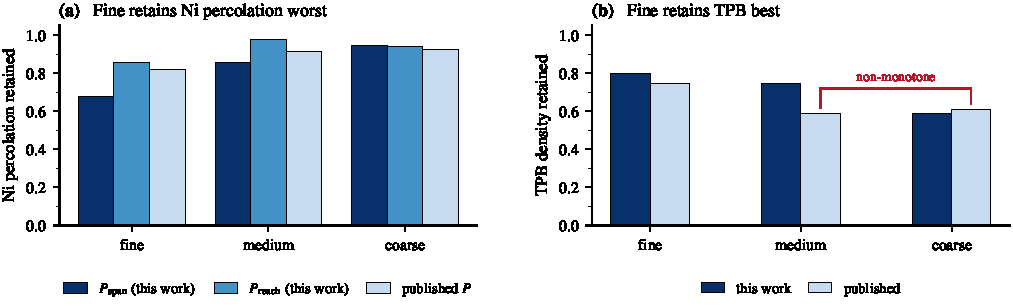
\includegraphics[width=\textwidth]{fig1_measured_signature.pdf}
  \caption{The measured signature the operators were built to reproduce.
  (a) Retained nickel percolation under three definitions. Fine is worst on
  all three; medium and coarse exchange places between $\Pspan$ and $\Preach$,
  so that comparison is treated as unresolved. (b) Retained TPB density. Fine
  is best in both series, but the published series is not monotone, so only
  the two-level statement is used. Data: \texttt{phase6\_comparison\_table.csv}.}
  \label{fig:signature}
\end{figure*}

\begin{table*}[tb]
  \centering
  \caption{Measured retention, degraded divided by pristine, on full stacks
  with no sub-sampling. Published values are from
  \cite{pecho2015transport,pecho2015tpb}. Pristine and degraded are different
  specimens. No dispersion is quoted because none exists to quote, each entry being a
single number computed once over an entire stack, not a mean over
  regions or seeds, so there is one measurement per anode per column. The
  region-to-region and seed-to-seed spreads reported elsewhere in this paper
  belong to the ROI-based graph metrics and to the damage operators, not to
  these quantities.}
  \label{tab:target}
  \begin{tabular}{lccccc}
    \toprule
    & \multicolumn{3}{c}{Ni percolation retained}
    & \multicolumn{2}{c}{TPB retained} \\
    \cmidrule(lr){2-4}\cmidrule(lr){5-6}
    anode & $\Pspan$ & $\Preach$ & published $P$ & this work & published \\
    \midrule
    fine   & \textbf{0.680} & 0.857 & 0.821 & \textbf{0.799} & 0.743 \\
    medium & 0.855 & 0.979 & 0.916 & 0.746 & 0.586 \\
    coarse & 0.947 & 0.942 & 0.924 & 0.590 & 0.608 \\
    \bottomrule
  \end{tabular}
\end{table*}

Table~\ref{tab:target} and Fig.~\ref{fig:signature} give the outcome. Our
absolute values track the published ones closely: $\Preach$ matches the
published $P$ to within \SIrange{0.1}{7.4}{\percent} on all six stacks. The
one fact that survives every definition is that the fine anode retains nickel
percolation worst, and it survives because the source papers state it
independently. The fine anode is simultaneously the best TPB retainer, which
is what makes the target interesting, since whatever mechanism destroys the
nickel
network in the finest structure leaves most of its reaction sites intact.

\subsection{A synthetic platform, and what it concealed}

Work began on a synthetic three-phase platform built from nickel spheres on a
jittered
regular lattice joined by explicit necks, with a particulate YSZ generator
whose sintering yield sets ceramic connectivity independently of grain size.
The platform passed a twelve-part qualification suite on volume fractions,
percolation, particle sizes, neck sizes, length-scale ordering and ceramic
fragility ordering. It was, by every check we thought to apply, a good
analogue.

Three mechanisms were tested on it and none produced the target ordering.
Widening the lower tail of the neck-size distribution by \num{1.33} and
\num{2.00} times at conserved nickel loading moved the bisection midpoint from
8.54 rounds to 8.50 and 8.50, a change of $-0.04$ rounds against a
pre-registered interpretability threshold of 1.0; 74 of 75 bisections returned
exactly 8.5. Severing every throat in the lower quartile of the size
distribution (100\% of candidates, at a cost of \SIrange{0.6}{5.3}{\percent}
of the nickel volume) produced no percolation failure whatever, with
$\Pspan=1.0000$ at the maximum intensity in 15 of 15 structures. Progressive
fracture of sintered YSZ contacts did separate the classes, by 2.87 rounds in
the predicted direction with non-overlapping seed ranges, and a
matched-fragility control in which pristine ceramic fragility was equalised
across classes inverted that separation to $-0.27$ rounds. The apparent
mechanism was pristine-state loading, since the class calibrated to start
nearest
its percolation threshold failed first, as it must. Without the control the
main-arm result would have read as a confident positive.

A graph audit run to explain the first two nulls found something more general
than the nulls themselves. The minimum source--sink cut of the synthetic
nickel network is exactly one complete lattice cross-section: 36, 25 and 16
edges for the three classes, which are $6^2$, $5^2$ and $4^2$, in every one
of fifteen structures, with zero seed-to-seed variance
(Fig.~\ref{fig:mincut}). A jittered regular lattice has no locally weak plane, because every cross-
section is statistically identical, so the minimum cut is a plane
and its size is fixed by the geometry rather than by the microstructure.
Removing half of all necks in random or increasing-area order still leaves
\SIrange{91}{97}{\percent} of the nickel in the spanning cluster, while a
targeted cut breaks medium at \SI{5.8}{\percent} of throats and coarse at
\SI{7.1}{\percent}, a factor of about eight apart. Fine cannot be broken by
neck removal at any budget. Jitter of 0.15 of the lattice pitch lets
neighbouring spheres approach to within less than their combined radii, so
\SI{13.1}{\percent} of fine's bonds are carried by direct sphere overlap
independent of their neck; severing the graph minimum cut leaves the voxel
mask spanning at exactly 1.0000 in all five seeds. The graph model understates
the platform's connectivity, and it understates it most for the class the
study needed to be most fragile. The critical edges overlap the lower-quartile
neck population at 0.250, 0.280 and 0.188 against a chance expectation of
0.25, which is why severing the narrow necks did nothing. In this architecture
the narrow necks are not load-bearing.

\begin{figure}[tb]
  \centering
  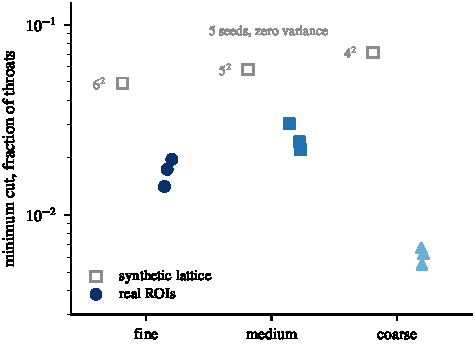
\includegraphics[width=\linewidth]{fig2_mincut.pdf}
  \caption{Minimum source--sink cut as a fraction of all throats, logarithmic
  axis. The synthetic lattice cuts at exactly one full cross-section, at the
  same fraction in all five structure seeds of each class. Real regions of
  interest cut at \SIrange{0.55}{0.67}{\percent} (coarse),
  \SIrange{1.41}{1.96}{\percent} (fine) and \SIrange{2.21}{3.02}{\percent}
  (medium) of throats, with region-to-region spread within every anode.
  Data: \texttt{audit\_ni\_vulnerability.csv},
  \texttt{c1real\_results.csv}.}
  \label{fig:mincut}
\end{figure}

The same audit measured the real networks for comparison. Real nickel networks
are disordered in a way the lattice is not, and connected-pair-distance
coefficients of variation of \numrange{0.38}{0.45}, coordination standard
deviations of \numrange{1.8}{2.9} against a lattice whose interior
coordination is fixed, and minimum cuts of a handful of edges rather than a
plane. It is the first of the failure modes, \textbf{a lattice minimum cut that is a
plane}, and it says what a synthetic platform
can be asked to do. A regular lattice cannot fail
the way a real network fails, and no local stochastic operator can make it do
so. Bond dilution does not help, because a diluted regular lattice remains
statistically homogeneous at large scale and the cut plane merely thins; the
property the lattice lacks is positional disorder, which cannot be created by
deleting bonds from a periodic grid.

That conclusion retracts the three mechanism results above, and we would
rather say so than leave them standing. The neck-widening and neck-severing
nulls are explained by the minimum-cut measurement, because an operator
confined to
the lower quartile of the throat distribution was attacking edges that carry
no more load than any other quartile, on a network that only a globally
coordinated cut can break. Those are nulls about the platform. The ceramic
fracture result is disqualified independently by its own matched-fragility
control. None of the three is evidence about real electrodes, and none is
counted as an eliminated mechanism anywhere in this paper. What survives from
the synthetic phase is the diagnosis of why it could not work.

The second failure mode, \textbf{a gate demanding perfect pristine
connectivity}, surfaced only when the operators were moved to real
data. Measured pristine spanning fractions per region are
0.9821/0.9754/0.9877 (fine), 0.9713/0.9446/0.9554 (medium) and
0.8878/0.9528/0.9157 (coarse). Between \SI{1.2}{\percent} and
\SI{11.2}{\percent} of the nickel in a real electrode is already disconnected
before service, and the disconnected fraction is coarseness-ordered. The
published percolation values carry the same message less sharply, at
\numrange{0.959}{0.985} rather than unity. Our synthetic qualification gate
required pristine $\Pspan$ to equal 1.0000 exactly, and every structure passed
it. That gate is unrepresentative of every real electrode measured here, and
it is what hid the next failure mode for the entire synthetic phase of the
work.

\subsection{The outcome metric rewrites its own denominator}
\label{sec:pruning}

The spanning fraction divides spanning-cluster voxels by total phase voxels,
which is how percolation is reported for this dataset and for electrodes
generally \cite{pecho2015transport}. Damage operators conventionally retain
only the largest connected component, on the physical grounds that isolated
nickel is electrically dead; the same reasoning underlies the standard
partition of electrode microstructure into active, dead-end and isolated
clusters \cite{chen2011}. Neither convention is ours and neither is wrong.
Together they are circular. Pruning deletes exactly the non-spanning voxels,
so after pruning the surviving component is the spanning one and
$\Pspan$ equals unity identically. The operator rewrites the denominator of
the metric used to judge it. It is the third failure mode, \textbf{pruning that fixes the spanning fraction
at unity}, and it took the longest to identify.

We state it as a finding rather than a slip because of how it behaved when we
tried to fix it. Our first diagnosis was that an oxidative dilation step was
bridging the disconnected fraction, which is physically plausible and would
have made this an operator defect with an operator remedy. We removed the
dilation step. The fine anode's TPB inflation moved from 15.24 to 14.80 and
$\Pspan$ remained exactly 1.0000 in all three anodes
(Fig.~\ref{fig:metric}a). The pathology survived a targeted, mechanistically
motivated repair, because the cause was the pruning step and not the
dilation.

Three properties make it hard to catch. The metric is correct on the pristine
structure, where across the nine regions it returns \numrange{0.888}{0.988}
rather than unity. It is
correct under any operator that does not prune. And on a test structure whose
qualification gate forces pristine $\Pspan$ to unity it is unobservable, since
the pruning step has nothing to delete. A group validating on synthetic
structures would pass every check either convention imposes alone and would
ship the combination.

The behaviour is identical in two independently implemented operators. On
real
regions, pristine $\Pspan$ of 0.9821, 0.9713 and 0.8878 becomes exactly 1.0000
at the first damage step in both.

\begin{figure*}[tb]
  \centering
  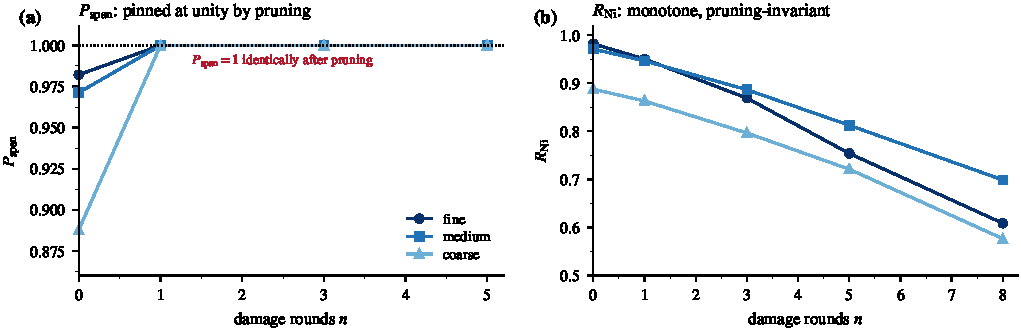
\includegraphics[width=\textwidth]{fig3_metric.pdf}
  \caption{(a) Spanning fraction under surface erosion on real regions of
  interest. Every anode reaches exactly unity at the first damage round and
  stays there, because largest-component pruning deletes the non-spanning
  voxels that form the denominator. (b) The pruning-invariant metric $\Rni$
  on the same runs declines monotonically from a pristine value that is not
  forced to unity. Data: \texttt{c1real\_o6\_validity.csv},
  \texttt{c1real\_rni\_gate.csv}.}
  \label{fig:metric}
\end{figure*}

This is a metric--operator incompatibility rather than an operator defect, and
the fix belongs to the metric. Scoring on spanning-cluster voxels as a
fraction of pristine nickel gives a quantity that does not move when
isolated material is deleted, falls monotonically under erosion
(Fig.~\ref{fig:metric}b), and is directly comparable to the measured retention
values. On the synthetic platform the pathology was invisible for a precise
reason. The qualification gate had forced pristine $\Pspan$ to unity, leaving
the pruning step nothing to remove.

\subsection{Voxel-scale moves manufacture TPB, whatever the operator's budget}

\begin{figure}[tb]
  \centering
  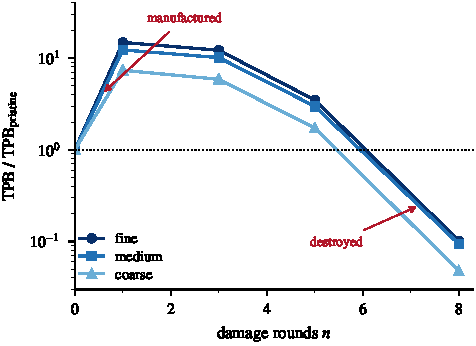
\includegraphics[width=\linewidth]{fig4_tpb.pdf}
  \caption{TPB density relative to pristine under surface erosion on real
  regions of interest. Stochastic single-voxel removal pits the nickel
  surface, and every new nickel/pore facet touching zirconia creates triple
  line. Any TPB conclusion drawn before the peak reports discretisation, not
  the electrode. Data: \texttt{c1real\_rni\_gate.csv}.}
  \label{fig:tpb}
\end{figure}

The fourth failure mode is in the same runs. \textbf{Voxel-scale moves
manufacture TPB}, inverting the quantity the
electrode is built around before destroying it. A voxel-scale operator does not
begin by removing triple line; it begins by manufacturing it, because removing
single voxels roughens a surface at the grid scale and every newly exposed
nickel/pore facet that happens to touch zirconia adds junction. Any TPB
conclusion drawn during that excursion reports the discretisation and not the
electrode.

The excursion is large. TPB density is multiplied by 14.8, 12.3 and 7.4 at the
first damage round before it collapses to \SIrange{4.8}{10.2}{\percent} of
pristine by the eighth (Fig.~\ref{fig:tpb}).

Removal is not the cause, and neither is a loose volume budget. A
volume-conserving redistribution operator run on synthetic structures showed
the same signature more mildly, raising nickel surface area by
\SIrange{1.4}{5.3}{\percent} at exactly conserved volume and roughly doubling
TPB, with per-class ratios of 2.02, 2.10 and 2.26. The sharper test is a
single-voxel swap that conserves volume exactly and decreases specific
surface area monotonically, run sequentially on the three real regions of
interest. It multiplies TPB density by 5.0, 4.9 and 3.7 for the fine, medium
and coarse anodes while satisfying both budgets throughout
(\texttt{o7\_gate\_a1v2\_real.py}). Neither conserving mass nor reducing area
prevents the artifact.

The reason is that the two quantities are not sensitive to the same thing.
Specific surface area is a facet count over the nickel/pore interface; TPB is a
one-dimensional junction count where three phases meet. Under the swap rule,
about \SI{80}{\percent} of accepted moves carry $\Delta A = 0$ exactly, which on
the fine anode is $207\,369$ of $258\,870$, and these are therefore unpriced by
an area criterion (Fig.~\ref{fig:gatetpb}b). An area budget does not constrain the
degree of freedom that governs TPB.

Where those unpriced moves land is worth measuring rather than assuming, and
the measurement is more specific than the guess. The rule removes nickel from
sites with few nickel neighbours, and nickel is thinnest against its own kind
exactly where it meets zirconia, since a voxel on that contact is backed by
ceramic rather than by more nickel. On the fine anode \SI{93.0}{\percent} of removed voxels are adjacent to YSZ, so
the operator is stripping nickel off the ceramic. Added material, by contrast, lands almost anywhere,
only \SI{3.3}{\percent} of it beside YSZ, and arrives as
\num{34500} fragments of median size two voxels.

Re-applying the two groups separately to the pristine structure separates their
contributions (Fig.~\ref{fig:counterfactual}). The contact-adjacent moves alone
reproduce the whole artifact, $\times 5.03$ against $\times 4.99$ for the full
set; every other move, which is \SI{97}{\percent} of the added material, gives
$\times 1.04$. The mechanism is therefore specific rather than diffuse. The area criterion
rewards precisely the moves that pit the nickel--zirconia contact patch, and the triple line lives on that patch's perimeter. The gate
prices the nickel/pore interface; the damage happens on the nickel/zirconia
interface, which the gate never inspects.

Forbidding those moves reduces the artifact without removing it, and the
residue is the more useful number. Tightening the rule to strict inequality,
$\Delta A < 0$, so that every accepted move must lower the area, leaves TPB
ratios of 1.53, 1.33 and 1.34 against 5.0, 4.9 and 3.7 under $\Delta A \leq 0$
(\texttt{o7\_strict\_inequality.py}). Most of the inflation is indeed the
neutral plateau; a third to a half of a doubling is not. Nor is a matched-budget
control needed to reach that conclusion. The greedy rule selects the smallest
$\nb(a)$ against the largest $\nb(b)$, so the extremal pair attains the minimum
$\Delta A$ available; if any strictly negative move exists, that pair is
strictly negative. Neutral moves are taken only once negative ones are
exhausted, so the first $M$ moves under $\Delta A \leq 0$ are exactly the $M$
moves the strict rule makes, and the two operators agree until the strict one
halts.

The consequence is that the criterion cannot be repaired by tightening it. A
strictly area-lowering operator still manufactures triple line, still raises
$\Rni$, and still never thins a neck. The problem is not that the area budget
admits a null space; it is that surface area is the wrong invariant to validate
a coarsening rule against, because a rule can satisfy it in full while moving
the microstructure away from the physics it is meant to represent.

That voxelised TPB estimates carry a resolution-dependent systematic bias is
established \cite{jorgensen2014,shimura2016}. What is different here is that the bias forms a large, non-monotone excursion
driven by the operator, rather than a fixed offset itself, so it cannot be cancelled by taking ratios to the
pristine state or by any calibration performed before damage. An operator
whose TPB retention exceeds unity is roughening rather than eroding, and this
is worth stating as a routine check, since it costs one line and it
disqualified
three operators here. On our synthetic platform the same excursion was
inconspicuous because the platform's absolute TPB was already about eightfold
too high, an artifact of synthetic phase placement rather than of the
estimator. On real data the corrected estimator returns
\numrange{4.48}{4.66}, \numrange{1.87}{2.37} and
\SIrange{1.47}{1.55}{\per\micro\metre\squared} for the three anodes against
published values of 3.62, 2.11 and 1.47, a factor of \numrange{1.0}{1.3}.

\subsection{Surface erosion reverses the measured ordering}

With a pruning-invariant metric and an operator that passes its remaining
validity checks, the mechanism test can finally be run. It fails, and it fails
in the wrong direction.

\begin{figure*}[tb]
  \centering
  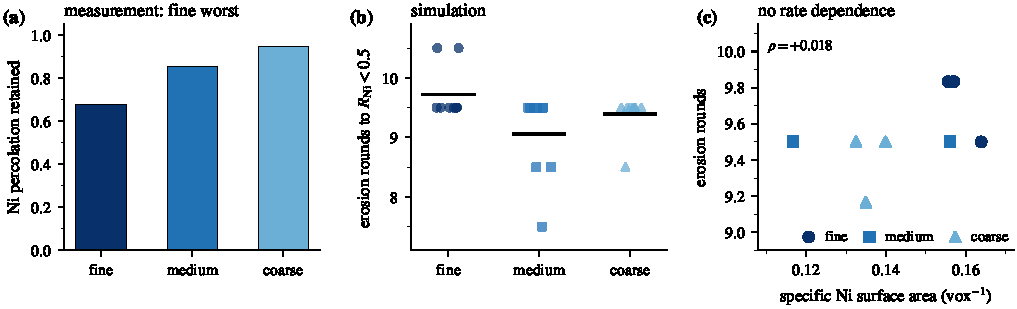
\includegraphics[width=\textwidth]{fig5_reversal.pdf}
  \caption{(a) Measured nickel percolation retention: fine is worst.
  (b) Erosion rounds to $\Rni<0.5$ on the same real microstructures, three
  regions and three damage seeds per anode; points are individual bisections
  and the horizontal bar is the class mean. Fine is the last anode to
  fail. (c) Transition
  against pristine specific nickel surface area, one point per region. Data:
  \texttt{c1real\_results.csv}, \texttt{phase6\_comparison\_table.csv}.}
  \label{fig:reversal}
\end{figure*}

\begin{figure}[tb]
  \centering
  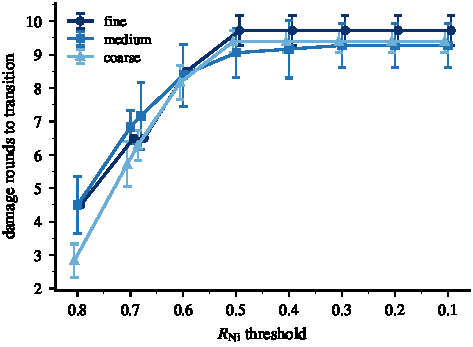
\includegraphics[width=\linewidth]{fig6_threshold_sweep.pdf}
  \caption{The reversal does not depend on where failure is declared. Damage
  rounds to transition against the $\Rni$ threshold, class means over three
  regions and three damage seeds, error bars one standard deviation. Every
  threshold is read from the same damage realisations, so the curves differ
  only in where the cut is placed. Nine thresholds are plotted; the unlabelled
  point between 0.70 and 0.60 is 0.68, the fine anode's own measured retention.
  Series are offset slightly in the threshold direction so that exact ties stay
  visible; fine and medium coincide at 4.50 rounds at a threshold of 0.80. The
  fine anode is the first to fail at none of the nine thresholds; the
  measurement says it should be first at all of them. The convergence below 0.50 is the discontinuous collapse of the
  spanning cluster: $\Rni$ crosses that whole range inside one round. Data:
  \texttt{o7\_threshold\_transitions.csv}.}
  \label{fig:threshold}
\end{figure}

The claim to be tested is a two-level one, because that is all the measurement
supports, which is that the fine anode retains nickel percolation worst and
therefore should
be the first to lose it. The simulation puts it last. That statement is the
result; the numbers below establish it and then establish that it does not
depend on where the failure threshold is placed.

Bisecting the damage intensity at which $\Rni$ falls below 0.50 gives class
means of 9.72 (fine), 9.06 (medium) and 9.39 (coarse) rounds; at 0.10 the
values are 9.72, 9.28 and 9.39. The pre-registered criterion required fine to
be lower than both others by at least one round. It is higher at both
(Fig.~\ref{fig:reversal}a,b).

The three-way ordering among those means should not be read, and we do not read
it. The separations are a few tenths of a round against region-to-region and
seed-to-seed standard deviations of 0.33 to 1.00, so which of medium and coarse
fails first is not resolved, exactly as medium versus coarse is unresolved in
the measurement itself.

What is resolved is the sign, and a threshold sweep shows it is not an artifact
of the pre-registered cut. Recording the full $\Rni$ curve over 20 rounds for
every region and seed, and reading nine thresholds from
\numrange{0.80}{0.10} off the same damage realisations, the fine anode is the
first to fail at none of them (Fig.~\ref{fig:threshold}). The identity of
the anode that does fail first changes with the threshold, being coarse above
0.60 and medium at and below 0.50, which is a further symptom of the unresolved
pair,
but fine is never among them. The sweep includes 0.68, the fine anode's own
measured retention, which is the threshold at which a placement artifact would
be most likely to show; it behaves like its neighbours.

Two incidental confirmations fall out. The five thresholds at and below 0.50
return an identical transition for the fine anode, 9.72 rounds in every case,
because $\Rni$ crosses that entire range within a single damage round; those
five were never five independent measurements. And the pre-registered pair of
thresholds, 0.50 and 0.10, sit inside that degenerate band, so the original
design had less resolution than its two-threshold form suggested.

Against the measurement, then, the operator inverts the one comparison the data
supports. Real retention makes fine the worst, and every simulated threshold
makes it the best or the middle.

Two candidate explanations were measured directly and neither survives. A
kinetic hypothesis predicts that the anode with the largest specific nickel
surface area erodes fastest; the raw Spearman coefficient is $+0.018$ at the
0.50 threshold and $+0.089$ at 0.10 (Fig.~\ref{fig:reversal}c). A topological
hypothesis predicts that the anode with the smallest minimum cut fails first;
the coefficients are $+0.028$ and $+0.213$. Nothing reaches the pre-registered
$|\rho|\geq0.6$, partial correlations controlling for pristine $\Pspan$ change
no sign that matters, and leave-one-out signs are inconsistent for three of
the four combinations.

The minimum-cut measurement produces a result worth separating from the null.
With the coarse regions properly sized at \SI{12}{\micro\metre}
(\numrange{258}{299} graph nodes, against \numrange{48}{72} in an earlier
under-sized pass), the coarse anode is by a wide margin the most topologically
fragile of the three, since its minimum cut fractions are
\numrange{0.0141}{0.0196} (fine), \numrange{0.0221}{0.0302} (medium) and
\numrange{0.0055}{0.0067} (coarse). On class means the coarse minimum-cut
fraction is 2.8 times below fine and 4.1 times below medium. Coarse is also
the best retainer in service, at 0.947, so pristine topological fragility runs
several-fold against the outcome it is supposed to predict. Taken with the
absent surface
area correlation, the sharpest statement this dataset supports about the
measured ordering says instead what does not control it, since neither the
pristine topology nor the specific surface area does.

Why the erosion operator behaves as it does is visible in the synthetic runs,
where the volume loss at the transition was recorded. Median across 45
bisections, fine loses \SI{74.4}{\percent} of its nickel before the network
breaks, medium \SI{70.5}{\percent} and coarse \SI{62.8}{\percent}. Fine does
erode faster, and its specific surface area really is the largest of the three
on real regions, 0.159 against coarse's 0.136, but its
network tolerates proportionally more volume loss before it stops spanning.
High specific surface area and high connectivity redundancy are both
consequences of fineness and they oppose each other in this outcome variable,
cancelling almost exactly.

\subsection{The area barrier}
\label{sec:barrier}

Surface erosion removes volume, whereas real coarsening conserves nickel and
reduces surface area. A removal-only operator also cannot reproduce the
measured change in nickel volume fraction, which is $-0.1006$, $-0.0164$ and
$+0.0145$ across the three anodes and therefore increases in the coarse
case. So the natural next operator is volume-conserving, and it is the one
that produces the most general result in this paper.

For a single-voxel swap on a 6-connected lattice the change in exposed nickel
area is exact rather than approximate. Removing a surface voxel $a$ changes
the count of exposed nickel faces by $2\,\nb(a)-6$, where $\nb$ counts nickel
neighbours, and adding a voxel at a pore site $b$ changes it by $6-2\,\nb(b)$.
Hence
\begin{equation}
  \Delta A = 2\,[\,\nb(a)-\nb(b)\,],
  \label{eq:dA}
\end{equation}
so that $\Delta A \leq 0$ if and only if $\nb(a) \leq \nb(b)$.
Material must leave a site with few nickel neighbours, which is convex and of
high curvature, and arrive at one with many, which is concave
(Fig.~\ref{fig:barrier}a). The expected direction of matter flow is recovered
without approximation.

\begin{figure*}[tb]
  \centering
  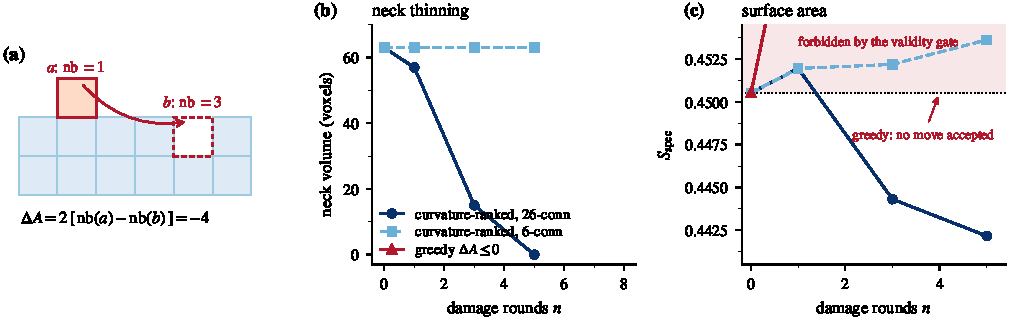
\includegraphics[width=\textwidth]{fig7_area_barrier.pdf}
  \caption{Two operators bracket an impossibility on a sphere--neck--sphere
  test body (neck 63 voxels, pristine $\Sspec = 0.45052$). (a) The exact area
  change of one swap on a 6-connected lattice, Eq.~\eqref{eq:dA}: moving a
  voxel from a protrusion to a notch lowers exposed area by four faces.
  (b) Neck volume. The curvature-ranked operator with a 26-connectivity
  stencil thins the neck to zero; with 6-connectivity it does nothing; the
  greedy operator leaves the neck intact. (c) Surface area. The
  curvature-ranked operator enters the region forbidden by its own validity
  criterion at $n=1$, at 0.45195 against a pristine 0.45052, before falling
  below pristine at $n=3$. The greedy operator accepts $96\%$ of proposals and
  also rises above pristine, to 0.46365 at $n=1$, because per-move
  $\Delta A\leq0$ guarantees do not compose across a batch ranked on a stale
  neighbour field. Data: \texttt{o5v2\_area\_barrier.csv}, regenerated by
  \texttt{o5v2\_regenerate.py}.}
  \label{fig:barrier}
\end{figure*}

A coarsening operator ought to reduce specific surface area, so requiring it
to do so monotonically is the criterion such a rule invites. We
pre-registered exactly that gate; we do not claim to have found it imposed
elsewhere, and its force here comes from being the check a careful
implementer would adopt, not from being a documented convention. Two move-selection rules were implemented against it and
they bracket the space of single-swap algorithms between them.

The first ranks candidate moves by a curvature proxy and applies them without
testing the area change. With a 6-connectivity stencil it does nothing useful,
leaving the model neck at 63 voxels; with a 26-connectivity stencil the neck
thins monotonically, 63 to 57 to 15 to 0, at exactly conserved volume
(Fig.~\ref{fig:barrier}b). The behaviour is genuinely Rayleigh-type, and it fails the gate, because at the first round the surface area rises, to
0.45195 against a pristine 0.45052, under both stencils
(Fig.~\ref{fig:barrier}c). Curvature rank is a proxy for the area change and
not the area change itself, because on a discrete lattice the added voxel
exposes new
faces at its own free sides, and at $n=1$ that transient exceeds the area
removed. By $n=3$ the added material has coalesced into the neck and the net
area falls below pristine. It is a fifth failure mode in its own right, \textbf{curvature rank is not the
area change}, and the one that
Eq.~\eqref{eq:dA} was derived to repair.

The second rule uses Eq.~\eqref{eq:dA} directly, accepting a swap only when
$\Delta A \leq 0$. It accepts $96\%$ of proposals on the test body, and it
still fails the gate, though not by refusing to move. Applied in batches of
$k = 0.03\,N_{\mathrm{surf}}$ per round, as implemented, the specific surface
area rises at every intensity, from $0.45052$ pristine to $0.46365$ at
$n=1$ and $0.46461$ at $n=5$. Equation~\eqref{eq:dA} is exact for one isolated
swap against a current neighbour field; a batch is ranked once against a stale
field, the moves interact, and the per-move guarantees do not sum.

Removing that confound does not rescue the rule. A strictly sequential
variant, in which one move is applied and the neighbour field recomputed before
the next, does lower the area, and on all three real electrodes it passes the
strict-decrease gate. Specific
surface area falls by \num{-0.00568}, \num{-0.00251} and \num{-0.00470} from
pristine values of 0.15696, 0.11670 and 0.13991 for the fine, medium and coarse
anodes, that is by \SIrange{2.2}{3.6}{\percent}, at exact volume conservation.
The rule is permissive rather than selective on real data, since essentially
every
extremal pair it examines is admissible, and it accepts until it runs out of
its move budget rather than out of legal moves. It fails
instead on two conditions that the synthetic test body could not probe, because
that body has no nickel--zirconia contact and does not span its domain, so its
triple-phase-boundary density and percolation are identically zero. On the real
regions of interest, triple-phase-boundary density rises by factors of
$5.0$, $4.9$ and $3.7$ for the fine, medium and coarse electrodes, and the
retained percolating fraction $R_{\mathrm{Ni}}$ rises rather than falls.

The mechanism is the area-neutral plateau. Roughly $80\%$ of accepted moves
carry $\Delta A = 0$ exactly, which on the fine electrode is $207\,369$ of
$258\,870$.
They are free under a surface-area criterion and are therefore unconstrained,
and they concentrate where nickel is thinnest against its own kind, which is
the contact with zirconia; \SI{93.0}{\percent} of removed voxels sit against
YSZ, and re-applying only those moves reproduces the entire inflation. A
monotone-area gate cannot detect this, because the area genuinely does decrease
while the microstructure degrades in a way the criterion does not measure.

The argument ends there, and its consequence is structural.
Rayleigh-type break-up of a solid cylinder by surface diffusion is a
collective, long-wavelength instability \cite{nichols1965}: a cylinder is
unstable to perturbations of wavelength greater than its circumference, but
the instability only lowers energy once a correlated set of voxels has moved
together, and any single-voxel perturbation raises the area first. One
operator crosses that barrier without pricing it and violates the criterion;
the other prices it and never crosses, spending its moves instead on the
zero-cost plateau, where they redistribute nickel without correlating. In no
variant, at any intensity, seed or move budget tested, did the neck thin, so
the
mechanism the rules exist to represent was never produced. A monotonicity gate
forbids the only bridge, finite-temperature acceptance of area-increasing
moves. Any single-voxel-swap coarsening study that both
enforces monotone surface-area reduction and claims to reproduce Rayleigh-type
neck break-up is therefore either not producing that break-up or is violating
its own validity criterion. The two cannot hold together. It is the sixth and most general of the failure modes, \textbf{area
monotonicity excludes the mechanism it validates}, and unlike the other five
it concerns what an operator class can represent rather than how a particular
implementation goes wrong.

\begin{figure*}[tb]
  \centering
  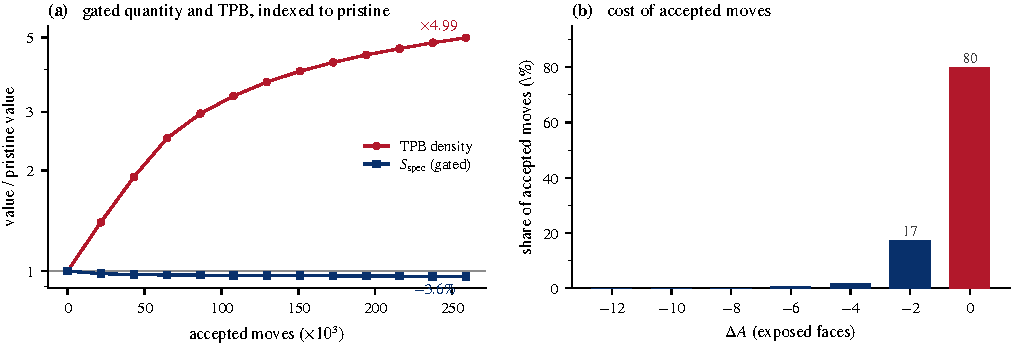
\includegraphics[width=\linewidth]{fig8_gate_vs_tpb.pdf}
  \caption{The validity criterion is satisfied while the quantity of interest
  is destroyed. Fine anode, \num{67} million voxels, sequential
  area-decreasing swap, volume conserved exactly. (a) Both quantities are
  divided by their pristine values so that they share one axis. Specific
  surface area, the gated quantity, falls \SI{3.6}{\percent}, while
  triple-phase-boundary density rises by a factor of $4.99$. (b) Why the gate
  does not object. Accepted moves by their cost in exposed faces; four in five
  carry $\Delta A = 0$ exactly and are unpriced by the criterion. Data:
  \texttt{o7\_trajectory.csv}, \texttt{o7\_da\_histogram.csv}.}
  \label{fig:gatetpb}
\end{figure*}

\begin{figure}[tb]
  \centering
  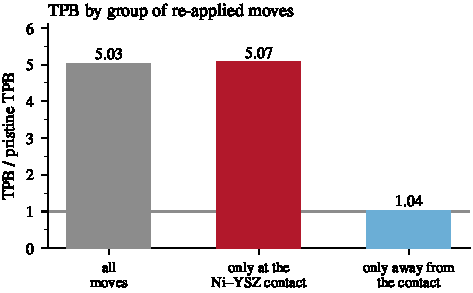
\includegraphics[width=\linewidth]{fig9_counterfactual.pdf}
  \caption{Where the triple-line inflation comes from, by re-applying the two
  groups of moves separately to the pristine structure. Moves that touch the
  nickel--zirconia contact reproduce the whole artifact on their own; every
  other move, \SI{97}{\percent} of the added material, changes TPB by four
  percent. Data: \texttt{o7\_counterfactual.csv}.}
  \label{fig:counterfactual}
\end{figure}

Its generality does not rest on the test body. Equation~\eqref{eq:dA} is exact
on any 6-connected lattice, and the local-minimum argument follows from two
facts of geometry rather than from this dumbbell, since a sphere minimises area
at
fixed volume, and a straight cylinder is stable against the displacement of
any individual voxel. The runs in Fig.~\ref{fig:barrier} demonstrate the
consequence on a case where the intended mechanism is unambiguous; they are
not what establishes it. The scope is correspondingly specific. The argument
covers operators that move one voxel at a time. It says nothing about
morphological openings and closings, block moves, or any update that
displaces a correlated set of voxels together, and a correlated update is
precisely what could cross the barrier.

What concealed this on the synthetic platform is straightforward, in that the
operator was
never asked to thin a neck against an explicit area budget, because the
structures were fully connected and the validation was about connectivity. We
stopped at this point, as the pre-registration required. The agglomeration
hypothesis is not falsified by any of this. It is untested, because the
operator class available to us cannot represent it under a gate we still
believe is the right gate for that operator class.

\subsection{Two hypotheses these data cannot pose}

Two further hypotheses were pre-registered with explicit untestability
branches, and both branches fired. We report them because a pre-registered
untestable outcome is information, and because the alternative of redefining
the criterion until a number emerges is the failure mode this paper is
about.

The first is redistribution, meaning nickel migrating from the
electrolyte-adjacent
functional layer into the support, most strongly in the finest microstructure.
Testing it requires an electrolyte interface to be present in both stacks of a
pair. The criterion, a sustained gradient of at least 0.05 in absolute
zirconia volume fraction between the two ends of a stack, is met in one pair
of three, and not in the fine anode, which is the anode the hypothesis
concerns, since gradients are 0.0042 and 0.0240 for fine in its two states,
0.0059
and 0.0552 for medium, and 0.1035 and 0.1157 for coarse. Nickel content does
vary strongly with depth in every stack, with coarse post-redox spanning 0.045 to
0.494 across \SI{0.5}{\micro\metre} slabs, but in fine and in pristine medium
that variation is not organised as a monotone interface gradient. It is
spatial heterogeneity, which is a different thing. The likeliest explanation
is prosaic. These sub-volumes are \SIrange{19}{24}{\micro\metre} across the
through-thickness direction against a support hundreds of micrometres thick,
and there is no reason a given tomogram must straddle the interface.

The second is cumulative-strain fracture of the ceramic scaffold, motivated by
the measured YSZ retention of 0.958, 0.865 and 0.000, in which the coarse
anode loses ceramic percolation outright. A deterministic operator broke YSZ
throats whose local redox strain, accumulated over cycles, exceeded a
threshold frozen before implementation. Both declared untestable conditions
fired. The coarse anode, which is the anode the hypothesis is about, yielded
no extractable YSZ throat graph at all. At a \SI{12}{\micro\metre} region the
YSZ phase does not span the transport axis, which is itself consistent with
coarse YSZ being the most fragmented phase in the dataset at a full-stack
pristine $\Pspan$ of 0.9246. And in the two anodes that did yield graphs the
operator is nearly inert, breaking \SIrange{1.0}{1.2}{\percent} of throats at
the maximum cycle count and moving YSZ retention to 0.9995 and 0.9996 against
targets of 0.958 and 0.865.

The diagnosis is a design lesson about pre-registration rather than about
nickel. The strain proxy is bounded above by the frozen strain scale
$\varepsilon_0 = 0.0065$, and after smoothing the per-throat values peak at
0.00413 and 0.00210. The frozen threshold of 0.010 sits above the maximum
single-cycle strain by factors of 2.4 and 4.8, so only cumulative
amplification lifts any throat over it. We froze an absolute threshold against
a quantity whose scale we had not yet measured. The remedy is to measure the
strain distribution on one region first and pre-register the threshold as a
quantile of it. We did not re-pick the threshold after seeing the
distribution, because doing so would be fitting a threshold to produce damage.
Independent support for the strain scale itself does exist. Reviews of redox
cycling report approximately \SI{1}{\percent} linear expansion on the first
complete oxidation of a Ni/YSZ composite \cite{sarantaridis2007}, against the
\SI{0.65}{\percent} we froze. The strain scale was therefore not the error,
though that does not rescue the run.

%======================================================================
\section{Discussion}
%======================================================================

\begin{table*}[tb]
  \centering
  \caption{The six failure modes, grouped by kind rather than by the order the
  work encountered them. Modes 1, 2, 3 and 5 are implementation faults. Each arises from a combination
of individually defensible choices, and each is removable by choosing
differently. Modes 4 and 6 are not. They are properties
  of what a voxel-scale move can do at a three-phase junction, and of what a
  monotone-area criterion admits, so they persist under any implementation of
  the move class. Numbering is retained from the text. Every mode was invisible
  on the synthetic platform for the reason given in the last column.}
  \label{tab:modes}
  \small
  \begin{tabular}{@{}c p{0.26\textwidth} p{0.31\textwidth} p{0.31\textwidth}@{}}
    \toprule
    & failure mode & what exposed it & what concealed it \\
    \midrule
    \multicolumn{4}{@{}l}{\emph{Implementation faults: individually reasonable
      conventions that go wrong in combination}}\\[2pt]
    1 & \textbf{lattice minimum cut is a plane} & cut is exactly $6^2$, $5^2$, $4^2$
      edges, zero variance & regular lattices were never asked to fail
      locally \\
    2 & \textbf{gate demands perfect pristine connectivity} & real electrodes carry
      \SIrange{1.2}{11.2}{\percent} isolated Ni & synthetic structures were
      built fully connected \\
    3 & \textbf{pruning fixes $\Pspan$ at unity} & $\Pspan$ jumps to 1.0000 at the
      first damage round & pristine $\Pspan$ was already 1.0000 by gate \\
    5 & \textbf{curvature rank $\neq$ area change} & $\Sspec$ rises at $n=1$ under
      both stencils & no explicit area budget was ever imposed \\[4pt]
    \multicolumn{4}{@{}l}{\emph{Structural limits: properties of the move class
      itself, which no implementation can remove}}\\[2pt]
    4 & \textbf{voxel moves manufacture TPB} & $7$--$15\times$ under erosion;
      $3.7$--$5.0\times$ under a volume- and area-budgeted swap & platform TPB
      was already $\sim8\times$ inflated \\
    6 & \textbf{area monotonicity excludes break-up} & $80\%$ of accepted moves are
      area-neutral; neck never thins & the operator was never asked to thin a
      neck \\
    \bottomrule
  \end{tabular}
\end{table*}

The six failure modes share a structure worth naming, set out in
Table~\ref{tab:modes}. In each case a modelling
convention that is individually reasonable becomes wrong in combination with
another, and the combination is invisible on the synthetic structures normally
used for validation. Retaining only the largest connected component is
reasonable; measuring the spanning fraction against total phase volume is
reasonable; together they are circular. Requiring perfect pristine
connectivity of a synthetic analogue is reasonable; it also removes the
condition under which that circularity would have been visible. Validating a
coarsening operator by monotone area reduction is reasonable; so is expecting
it to reproduce capillary break-up; together they are contradictory. A regular
lattice is a reasonable test structure; a stochastic local operator is a
reasonable model of degradation; together they cannot produce a percolation
failure, because the lattice's minimum cut is a plane and local action cannot
find one.

The prescription that follows is narrower and cheaper than a general appeal to
rigour. Validation criteria and mechanisms should be checked
against each other explicitly, and preferably on structures that are imperfect
in the way real ones are. Three of the six modes above would have been caught
by a test structure that was merely not fully connected, and a fourth
by asking whether the operator can in principle produce the move the mechanism
requires. A synthetic object that is fully connected, periodic and smooth will
pass suites that a real microstructure fails, and it will conceal precisely
the interactions that matter.

\subsection{Relation to continuum and discrete prior work}

The impossibility of Section~\ref{sec:barrier} is specific to voxel-swap
operators validated by monotone area reduction, and it does not extend to
continuum formulations. A phase-field model evolves a continuous order
parameter under a free-energy functional and is not restricted to single-voxel
moves, so it can pass through the transient area increase that a discrete swap
cannot. The alternative is not hypothetical for this material, since
phase-field
simulations of Ni coarsening have been run on three-dimensional Ni--YSZ
reconstructions from ptychographic nano-tomography with measured
thermophysical inputs \cite{yang2023}, validated against ex-situ imaging of
annealed specimens \cite{trini2021}, and coupled to performance models on
FIB-SEM reconstructions \cite{hoffrogge2023}, in a line going back to the
three-phase simulations of Chen and co-workers \cite{chen2011}. That body of
work is the appropriate point of comparison, and it sharpens the present claim
rather than weakening it. Where a study needs coarsening, a continuum
formulation is the sound choice. Where a study uses discrete voxel operators,
as many connectivity and TPB studies do because they act directly on the
segmented label field, the compatibility check of Eq.~\eqref{eq:dA} should be
run before any validity gate is adopted.

Discrete lattice methods are not thereby disqualified for this material
either, and the clearest evidence is a model that makes the same move we do. A
Potts kinetic Monte Carlo treatment of NiO--YSZ sintering, calibrated and
validated against FIB-SEM microstructure \cite{zhou2023}, represents surface
diffusion as the exchange of a pore site with a neighbouring solid site, so
that a
single-voxel swap on a voxel grid, which is our move class on our
discretisation. It reaches the coarsening behaviour our operator could not.
The difference is the acceptance rule. That model accepts a swap that raises
the system energy with probability $\exp(-\Delta E / k_{\mathrm{B}}T)$ at a
simulation temperature, so the barrier of Eq.~\eqref{eq:dA} is crossed rather
than avoided.

The distinction that matters is therefore not continuum against discrete, and
not even swap against non-swap. It is whether energy-raising moves are
permitted at all. A monotone area-reduction gate forbids them, and it forbids
them as a validity criterion rather than as a choice of dynamics. The impossibility is narrow for that reason, and easy to walk into for the
same one, since the
gate looks like rigour and functions like a constraint on the physics. The
same gate imposed on the model of \cite{zhou2023} would forbid the
energy-raising moves its Metropolis rule depends on; that follows from the
definition of the gate rather than from any run of ours, and no such gate is
imposed there.

The comparison should be pressed past the sixth mode, because it does not stop
there. Of the six in Table~\ref{tab:modes}, that model is structurally exposed
to one. Mode 4 as generalised above is a property of voxel-scale moves at a
three-phase junction rather than of any particular acceptance rule, and a Potts
model on a voxel grid makes voxel-scale moves; it is therefore subject to the
same transient inflation of triple line, and a study using one should check
that its TPB trajectory does not exceed unity before reading anything from it.
What that model does avoid is the persistent pathologies. It
takes real reconstructions as input, so there is no jittered lattice with a
planar minimum cut and no qualification gate demanding perfect pristine
connectivity. It scores on volume fraction, specific surface area, tortuosity
and TPB density rather than on a spanning fraction, so the circularity of the
third mode has nothing to act on. Its evolution is driven by an energy
functional rather than by stochastic voxel removal, so the roughening of the
fourth does not arise, and it evaluates that energy explicitly rather than
through a curvature proxy, which is the fifth. Three choices account for all
six: real input, an explicit energy, and finite-temperature acceptance. We
made none of them.

We take that as the strongest available support for the prescription of this
section rather than as an argument against it. The six modes are not exotic.
They are what a study meets when it declines one or more of those three
choices, and a reader is entitled to conclude that the established formulation
should have been the starting point. What this paper adds is a measurement of what the worse method costs, the
existence of the better one being already established.
Nothing in \cite{zhou2023} reports the effect of an area-monotonicity gate on
a swap operator, because no such gate is imposed there.
Equation~\eqref{eq:dA}, the area-neutral plateau and the bracketing pair of
operators are a quantitative account of a trap that a well-designed study
walks around without comment, and the value of documenting a trap does not
depend on its being unavoidable.

Two of our six modes have partial precedent and we do not claim them as new.
The systematic error in TPB length computed from voxelised data is documented,
both as a function of calculation rule \cite{jorgensen2014} and of imaging
resolution \cite{shimura2016}; what we add is that a damage operator turns
that static bias into a large non-monotone excursion that no pre-damage
calibration removes. That real electrodes contain isolated nickel is likewise
known, and appears in the source papers for this dataset as pristine
percolation values below unity \cite{pecho2015transport}; what we add is the
consequence, that a qualification gate demanding perfect pristine connectivity
disqualifies the synthetic analogue as a place to discover metric pathologies.
The remaining four (the pruning circularity, lattice minimum-cut planarity,
the curvature-proxy failure and the area barrier) we have not found stated
elsewhere, which is a statement about our search rather than a claim of
priority.

\subsection{What the negative result does and does not establish}
\label{sec:limits}

One operator class reached a mechanism verdict on real microstructures and
reversed the measured ordering. The three synthetic mechanism tests are
withdrawn with the platform that carried them. We have not shown that no
geometric mechanism reproduces the ordering, and on the strength of one
operator class on real data we could not. We have specifically not shown that agglomeration is not the
physical cause of nickel percolation loss: Section~\ref{sec:barrier} says we
could not test agglomeration with this operator class under this gate, which
is a statement about the method and not about the material. Nor is anything
here evidence against continuum or phase-field treatments, which are subject
to none of the six modes.

The limitations are the ordinary ones and they bind hard. There are three
anodes, three regions of interest per anode and three damage seeds, so class
comparisons are correspondingly weak, although the sign reversal in
Fig.~\ref{fig:reversal} is consistent across all nine regions. Pristine and
degraded stacks are different specimens, so every retention magnitude carries
specimen variation and no paired quantity is available. The limitation belongs to this dataset rather than to the problem, because
ex-situ tomography of a single
specimen imaged before and after annealing has been done on this material
\cite{trini2021}, and it is what a repeat of this work should be built on.
The two $\Rni$
thresholds are not independent, because the spanning cluster vanishes
discontinuously and $\Rni$ crosses 0.50 and 0.10 within one round in most
regions, which is itself a finding about how percolation fails in these
structures. Regions are single-scale at 8 or \SI{12}{\micro\metre}, the coarse
anode being bounded above by a stack that is only \SI{13.3}{\micro\metre}
deep. Graph metrics use frozen watershed parameters. Coarse YSZ throats have a
tenth-percentile inscribed diameter of roughly two voxels, below this
project's four-voxel resolution floor, so any throat-targeted ceramic fracture
rests partly on sub-resolution features.

Four further limitations are specific enough to name. First, the region sizes
were set by the nickel graph and not by the ceramic. The \SI{12}{\micro\metre}
coarse region was chosen to clear a 150-node floor for the nickel network, and
the same choice over-resolves the YSZ phase, whose contacts are far finer; the
anode where a ceramic-fracture mechanism would matter most is therefore the one
where our sampling suits it least. The sizes also happen to hold the voxel
count near $400^3$ across the three anodes, which was a computational
convenience and not a representativeness argument. Second, the synthetic
generator was recalibrated once against the measured connectivity of its own
contact graph, which is an internal consistency check rather than a comparison
with FIB-SEM minimum cuts or triple-phase-boundary distributions; the platform
was never shown to reproduce those external quantities, which is part of why
its results did not survive contact with real data. Third, connectivity is
evaluated throughout at 6-connectivity. The convention is the conservative one, but it ignores face-diagonal
contacts, and the effect is not neutral across the
series, because the finest anode has the most surface per unit volume and
therefore the
most opportunity for such contacts, so its pristine connectivity is the most
likely to be understated. That reasoning is correct in direction and negligible
in size. Recomputing the pristine spanning fraction under 26-connectivity on
all nine regions moves the fine anode by $+0.0004$ on the class mean and the
medium and coarse anodes by nothing at all, to four decimal places
(\texttt{o7\_connectivity\_check.csv}). The disconnected nickel fraction is
unchanged at \SI{1.8}{\percent}, \SI{4.3}{\percent} and \SI{8.1}{\percent}. The
convention favours the fine anode as predicted and by an amount that changes no
statement in this paper. Fourth, regions are cut with free, non-periodic boundaries, which
truncate particles at the faces. That penalty also falls unevenly, bearing
hardest on the anode whose particles are smallest relative to the region, again
the fine one. Both conventions push in the same direction on the same sample,
and both are frozen rather than tuned, but neither was varied.

Three further conventions are recorded because they bear on how the evidence
should be read rather than on the numbers themselves. The demonstration of the
curvature-rank mode applies \num{61} moves per round from a single ranking, so
its measured area rise is confounded with the batching that mode~6 identifies;
the analytic point, that a curvature rank is not $\Delta A$, does not depend on
that measurement. Operators differ in whether domain-face voxels may move, in
that the
sequential rule excludes them, the batched one does not, which matters most for
the smallest regions. And the erosion operator retains only the largest
connected component, which is not guaranteed to be nested across rounds if the
largest component ever changes identity; it does not do so here, all 27
recorded $\Rni$ curves being monotone, but the guarantee is empirical rather
than structural.

The open question is not which operator to try next. It is what class of
mechanism could produce loss of long-range nickel connectivity together with
retention of most of the reaction sites, which is what \SI{80}{\percent} TPB
retention at \SI{68}{\percent} percolation retention means in the fine anode.
Uniform removal thins everything at once and eliminates both together; our
synthetic runs destroy \SI{99.5}{\percent} of TPB by the time nickel
percolation is lost, some 164 times more than the real anode does. Dewetting
and retraction of nickel into compact particles would break long-range
connectivity while comparatively preserving the nickel/zirconia contact
perimeter where TPB lives. We record it as an untested possibility rather than
a surviving candidate, since nothing here eliminates its competitors and no run
in
this work either supports or excludes it.

Two claims must be separated here, because only one of them fails. That a
greedy operator is frozen, and therefore cannot reach the mechanism, is
withdrawn, since once corrected it accepts almost every move. The impossibility
above is
untouched, because it turns on which moves are permitted, not on how
many are taken. No single-voxel-swap operator respecting monotone area
reduction thinned a neck at any intensity, seed, move budget or acceptance rule
tried, strictly area-lowering or finite-temperature. The one variant that did
thin it, curvature ranking under a 26-connectivity stencil which reached zero
neck volume by $n=5$, violated the area criterion at its first step, at
0.45195 against a pristine 0.45052. Thinning and the criterion were never
observed together.

Two qualifications keep that honest. Lifting the restriction is necessary but
not sufficient, since the finite-temperature runs permit area-increasing moves
and
still produce surface roughening rather than break-up. And the impossibility is
analytic only for a strictly decreasing criterion. Under the non-strict form
the $\Delta A = 0$ plateau is admissible and large, so a monotone rule is free
to wander it; that such wandering does not reach break-up is established here
empirically, over some $2.6\times10^{5}$ accepted moves, rather than proved.

The practical consequence stands. If the anticorrelation is to be explained by
Rayleigh-type break-up, testing that explanation requires a formulation not
restricted to monotone area reduction. The condition is one on the method and not a recipe for the mechanism, and the
anticorrelation itself remains
an open puzzle this class of operator cannot pose.

%======================================================================
\section{Conclusions}
%======================================================================

\begin{enumerate}
\item Enforcing monotone surface-area reduction as a validity criterion
  structurally excludes Rayleigh-type neck break-up. On a 6-connected lattice
  the criterion reduces to $\nb(a)\leq\nb(b)$, which leaves a large
  area-neutral plateau, in which roughly $80\%$ of accepted moves carry
  $\Delta A = 0$, are unpriced by the criterion, and redistribute nickel
  without correlating into an instability. A greedy area-decreasing operator
  therefore accepts almost every move, never thins a neck, and---on real
  electrodes---inflates TPB density four- to five-fold while satisfying the
  area criterion it is validated against. The exclusion is analytic for a
  strictly decreasing criterion, where no admissible move can go uphill; under
  the non-strict form it rests on the plateau argument together with the
  measurement, and is stated at that strength. The criterion and the mechanism
  were never honoured together by any single-swap operator tested here.
\item Five further failure modes were measured, each invisible on synthetic
  test structures. Largest-component pruning makes the spanning fraction
  identically unity; voxel-scale moves multiply TPB density by 7 to 15 under
  erosion and by 3.7 to 5.0 under a swap that conserves volume and reduces
  area, so neither budget protects the estimate; qualification gates demanding perfect pristine
  connectivity are unrepresentative of electrodes carrying
  \SIrange{1.2}{11.2}{\percent} disconnected nickel; a jittered regular
  lattice cuts at exactly one full cross-section with zero variance, whereas
  real networks cut at \SIrange{0.5}{3}{\percent} of throats; and
  curvature-ranked moves do not deliver the area reduction assumed of them.
\item Stochastic surface erosion applied to real microstructures with a
  pruning-invariant metric reverses the measured degradation ordering, since
the
  fine anode is the last to lose percolation rather than the first.
\item Under the uniform surface-erosion operator tested here, neither pristine
  topology nor specific nickel surface area predicts the measured ordering.
  The coarse anode carries the smallest minimum cut of the three, 2.8 times
  below fine and 4.1 times below medium on class means, and is the best
  retainer in service. The scope of that statement is the operator, not
  degradation in general, because a rule with a different spatial bias could rank
them
  differently, and none was tested.
\item Real nickel networks fail at \SIrange{0.5}{3}{\percent} of throats
  through small, region-variable, non-planar cuts, against a lattice that
  fails at \SIrange{4.9}{7.1}{\percent} and always through a full
  cross-section. A synthetic generator intended to reproduce real behaviour
  must carry comparable positional disorder, meaning coordination standard
deviation
  \numrange{1.8}{2.9} and a connected-pair-distance coefficient of variation
  of \numrange{0.38}{0.45}.
\end{enumerate}

%======================================================================
\section*{CRediT authorship contribution statement}
%======================================================================

\textbf{Arnav Mehta}: Conceptualization, Methodology, Software, Validation,
Formal analysis, Investigation, Data curation, Writing -- original draft,
Writing -- review and editing, Visualization.

%======================================================================
\section*{Declaration of competing interest}
%======================================================================

The author declares that he has no known competing financial interests or
personal relationships that could have appeared to influence the work reported
in this paper.

%======================================================================
\section*{Funding}
%======================================================================

This research did not receive any specific grant from funding agencies in the
public, commercial, or not-for-profit sectors.

%======================================================================
\section*{Data and code availability}
%======================================================================

\begingroup\sloppy
All code, pre-registration documents, run reports and result tables are in the
project repository, \url{https://github.com/mehtaarnav/voxel-damage-operators-niysz}.
The exact state that produced every number in this paper is archived at
\url{https://doi.org/10.5281/zenodo.21969406}; the concept identifier
\url{https://doi.org/10.5281/zenodo.21969405} resolves to the latest version.
The tomography data itself is third-party and is not redistributed there; it is
the Holzer/Pecho Ni--YSZ FIB-tomography dataset at
\url{https://zenodo.org/records/4056538}, fetched by the download script into a
directory that is deliberately not committed.
Every number in this paper
traces to a committed CSV: the measured signature to
\texttt{out/phase6/phase6\_comparison\_table.csv}; the erosion bisections,
minimum cuts and Spearman inputs to \texttt{out/project2/c1real\_results.csv};
the metric and TPB behaviour to \texttt{c1real\_o6\_validity.csv} and
\texttt{c1real\_rni\_gate.csv}; the lattice audit to
\texttt{audit\_ni\_vulnerability.csv}; the synthetic mechanism tests to
\texttt{out/platform\_v2/p10\_group\_experiment.csv} and
\texttt{out/project2/step2\_O2\_ceiling\_check.csv},
\texttt{step2\_O3\_main.csv}, \texttt{step2\_O3\_control.csv}; the synthetic
volume loss at the erosion transition to \texttt{step2\_O1\_main.csv} and the
redistribution operator's surface and TPB ratios to
\texttt{step2\_O5\_ceiling\_check.csv}; the
volume-conserving gate to \texttt{o5v2\_area\_barrier.csv}; the redistribution
and ceramic-fracture branches to
\texttt{h1\_depth\_profiles.csv}, \texttt{h1\_layer\_summary.csv} and
\texttt{csfm\_results.csv}; and the implementation-validation constants to
\texttt{validation\_constants.csv}. The last two of those are transcriptions,
by \texttt{scripts/project2/o5v2\_transcribe.py} and
\texttt{transcribe\_validation.py}, of values that their runs reported in
markdown rather than in a table; each row carries the report it came from.
Figures regenerate with
\texttt{python scripts/project2/make\_figures.py}, and file names match the
figure numbers.

Each pre-registration was committed before the run it governed and the chain
of commits is recorded in the repository. Corrections made against our own
earlier results during the work, among them a TPB estimator that over-counted
fourfold
through periodic wrap, reversed axis extents that made one audit's cut
fractions provisional until re-run, a validity check that never compared
against the pristine state and printed a pass on a failing run, a
pre-registered secondary-outcome rule that selected a saturating measurement
point, an internally contradictory plan specifying both Metropolis acceptance
and strict area monotonicity, and the one that changed a headline result, a
neighbour count taken with a structuring element that includes the
centre voxel, which biased a comparison across two voxel populations by one and
made an operator that accepts \SI{96}{\percent} of proposals appear to accept
none, are all logged in the run reports at the point where each was found. Two
further specifications were found to be load-bearing rather than incidental
and are now part of the operator definition rather than of its implementation:
sequential rather than batched application, and random rather than
insertion-order tie-breaking among moves of equal $\Delta A$.
\endgroup

%======================================================================
\begin{thebibliography}{99}

\bibitem{simwonis2000}
D.~Simwonis, F.~Tietz, D.~St\"over,
Nickel coarsening in annealed Ni/8YSZ anode substrates for solid oxide fuel
cells,
Solid State Ionics 132 (3--4) (2000) 241--251.

\bibitem{sarantaridis2007}
D.~Sarantaridis, A.~Atkinson,
Redox cycling of Ni-based solid oxide fuel cell anodes: a review,
Fuel Cells 7 (3) (2007) 246--258.

\bibitem{monaco2019}
F.~Monaco, M.~Hubert, J.~Vulliet, J.~P. Ouweltjes, D.~Montinaro, P.~Cloetens,
P.~Piccardo, F.~Lefebvre-Joud, J.~Laurencin,
Degradation of Ni--YSZ electrodes in solid oxide cells: impact of polarization
and initial microstructure on the Ni evolution,
Journal of The Electrochemical Society 166 (15) (2019) F1229--F1242.

\bibitem{chen2011}
H.-Y. Chen, H.-C. Yu, J.~S. Cronin, J.~R. Wilson, S.~A. Barnett, K.~Thornton,
Simulation of coarsening in three-phase solid oxide fuel cell anodes,
Journal of Power Sources 196 (2011) 1333--1337.

\bibitem{trini2021}
M.~Trini, S.~De~Angelis, P.~S. J{\o}rgensen, P.~V. Hendriksen, K.~Thornton,
M.~Chen,
Towards the validation of a phase field model for Ni coarsening in solid oxide
cells,
Acta Materialia 212 (2021) 116887.

\bibitem{yang2023}
S.~Yang, J.~Gao, M.~Trini, S.~De~Angelis, P.~S. J{\o}rgensen, J.~R. Bowen,
L.~Zhang, M.~Chen,
Ni coarsening in Ni--yttria stabilized zirconia electrodes: three-dimensional
quantitative phase-field simulations supported by ex-situ ptychographic
nano-tomography,
Acta Materialia 246 (2023) 118708.

\bibitem{hoffrogge2023}
P.~W. Hoffrogge, D.~Schneider, F.~Wankm\"uller, M.~Meffert, D.~Gerthsen,
A.~Weber, B.~Nestler, M.~Wieler,
Performance estimation by multiphase-field simulations and transmission-line
modeling of nickel coarsening in FIB-SEM reconstructed Ni--YSZ SOFC anodes I:
influence of wetting angle,
Journal of Power Sources 570 (2023) 233031.

\bibitem{zhou2023}
S.~Zhou, X.~Liu, Z.~Yan, S.~Hara, N.~Shikazono, Z.~Zhong,
Kinetic Monte Carlo (KMC) simulation of sintering of nickel oxide--yttria
stabilized zirconia composites: model, parameter calibration and validation,
Materials \& Design 232 (2023) 112094.

\bibitem{pecho2015transport}
O.~M. Pecho, O.~Stenzel, B.~Iwanschitz, P.~Gasser, M.~Neumann, V.~Schmidt,
M.~Prestat, T.~Hocker, R.~J. Flatt, L.~Holzer,
3D microstructure effects in Ni--YSZ anodes: prediction of effective transport
properties and optimization of redox stability,
Materials 8 (9) (2015) 5554--5585.

\bibitem{pecho2015tpb}
O.~M. Pecho, A.~Mai, B.~M\"unch, T.~Hocker, R.~J. Flatt, L.~Holzer,
3D microstructure effects in Ni--YSZ anodes: influence of TPB lengths on the
electrochemical performance,
Materials 8 (10) (2015) 7129--7144.

\bibitem{herring1950}
C.~Herring,
Effect of change of scale on sintering phenomena,
Journal of Applied Physics 21 (4) (1950) 301--303.

\bibitem{wang2013}
J.~Wang, Z.~Zhou, W.~Zhang, T.~M. Garoni, Y.~Deng,
Bond and site percolation in three dimensions,
Physical Review E 87 (2013) 052107; erratum Physical Review E 89 (2014)
069907.

\bibitem{gostick2017}
J.~T. Gostick,
Versatile and efficient pore network extraction method using marker-based
watershed segmentation,
Physical Review E 96 (2017) 023307.

\bibitem{jorgensen2014}
P.~S. J{\o}rgensen, K.~Yakal-Kremski, J.~Wilson, J.~R. Bowen, S.~Barnett,
On the accuracy of triple phase boundary lengths calculated from tomographic
image data,
Journal of Power Sources 261 (2014) 198--205.

\bibitem{shimura2016}
T.~Shimura, Z.~Jiao, N.~Shikazono,
Dependence of solid oxide fuel cell electrode microstructure parameters on
focused ion beam -- scanning electron microscopy resolution,
International Journal of Hydrogen Energy 41 (48) (2016) 22373--22380.

\bibitem{lorenz1998}
C.~D. Lorenz, R.~M. Ziff,
Precise determination of the bond percolation thresholds and finite-size
scaling corrections for the sc, fcc, and bcc lattices,
Physical Review E 57 (1998) 230--236.

\bibitem{nichols1965}
F.~A. Nichols, W.~W. Mullins,
Morphological changes of a surface of revolution due to capillarity-induced
surface diffusion,
Journal of Applied Physics 36 (6) (1965) 1826--1835.

\end{thebibliography}

\end{document}
